\documentclass[letterpaper,  %a4paper
               %boxit,
               %titlepage,   % separate title page
               %refpage      % separate references
              ]{jacow-2_3}   %jacow}
%
% CHANGE SEQUENCE OF GRAPHICS EXTENSION TO BE EMBEDDED
% ----------------------------------------------------
% test for XeTeX where the sequence is by default eps-> pdf, jpg, png, pdf, ...
%    and the JACoW template provides JACpic2v3.eps and JACpic2v3.jpg which
%    might generates errors, therefore PNG and JPG first
%
\makeatletter%
	\ifboolexpr{bool{xetex}}
	 {\renewcommand{\Gin@extensions}{.pdf,%
	                    .png,.jpg,.bmp,.pict,.tif,.psd,.mac,.sga,.tga,.gif,%
	                    .eps,.ps,%
	                    }}{}
\makeatother

% CHECK FOR XeTeX/LuaTeX BEFORE DEFINING AN INPUT ENCODING
% --------------------------------------------------------
%   utf8  is default for XeTeX/LuaTeX 
%   utf8  in LaTeX only realizes a small portion of codes
%
\ifboolexpr{bool{xetex} or bool{luatex}} % test for XeTeX/LuaTeX
 {}                                      % input encoding is utf8 by default
 {\usepackage[utf8]{inputenc}}           % switch to utf8

\usepackage[USenglish]{babel}			 

\usepackage[final]{pdfpages}
\usepackage{multirow}
\usepackage{ragged2e}
\usepackage{tikz}
\usetikzlibrary{shapes,arrows,snakes,backgrounds}
\usetikzlibrary{mindmap,trees}
\usetikzlibrary{decorations.pathreplacing}
\usetikzlibrary{plotmarks}
%
% if BibLaTeX is used
%
\ifboolexpr{bool{jacowbiblatex}}%
 {%
  \addbibresource{jacow-test.bib}
  \addbibresource{biblatex-examples.bib}
 }{}
\listfiles

\newcommand\SEC[1]{\textbf{\uppercase{#1}}}

\begin{document}

\title{Staged Two Beam Acceleration Beam Line Design for the AWA Facility}

\author{N. Neveu\thanks{nneveu@anl.gov}\textsuperscript{1}, 
	    L. Spentzouris, Illinois Institute of Technology, Chicago, IL, USA \\
	    J. G. Power, W. Gai \textsuperscript{1}Argonne National Laboratory, Lemont, IL, USA \\
	    C. Jing, Euclid Techlabs LLC, Solon, OH, USA}
\maketitle

%
\begin{abstract}
Two beam acceleration is a candidate for future high energy physics machines and FEL user facilities. 
This scheme consists of two independent electron beam lines operating synchronously. 
High-charge, 70 MeV drive bunch trains are injected from the rf photoinjector into
decelerating structures to generate a few hundred MW of rf power. 
This rf power is transferred through an rf waveguide to accelerating structures that are used to
accelerate the witness beam. Staging refers to the sequential acceleration (energy gain) 
in two or more structures on the witness beam line. A kicker was incorporated on the 
drive beam line to accomplish a modular design so that each accelerating structure 
can be independently powered by a separate drive beam. 
Simulations were performed in OPAL-T to model the two beam lines. 
Beam sizes at the center of the structures was minimized to ensure good charge transmission. 
The resulting design will be the basis for proof of principle experiments that will take place 
at the Argonne Wakefield Accelerator (AWA) facility.
\end{abstract}


\section{AWA Facility}
The AWA facility houses two rf photoinjectors
operating at \SI{1.3}{GHz}. 
The bunch charge is routinely adjusted for depending on the requirements 
of the experiments downstream of the photoinjector.
Typical operating charges are 1, 4, 10, and \SI{40}{nC}. 
While these are the most
common operating modes, other charges have been requested 
and provided depending on the experiment.
Recent experiments include emittance exchange \cite{eex}, 
high gradient structure tests \cite{pets}, thermal emittance measurements \cite{therm}, 
and two beam acceleration \cite{tba} (TBA), which is the subject of this proceeding. 

\section{Two Beam Acceleration Layout}
The AWA facility lends well to TBA experiments due to the 
close proximity of both operational photoinjectors. 
They are located in the same bunker and located about two meters apart.
This number slightly varies depending on which part of the beam 
lines you are comparing. For the remainder of this paper, we will
refer to the low charge beam line as the "witness" line, 
and the high charge, beam line as the "drive" line.
While the charge on each line can be varied, for TBA experiments, 
the witness line is operated at \SI{1}{nC} and the drive line
is operated at \SI{40}{nC}.

The planned TBA layout is shown in Fig.~\ref{beamline}.
The drive line has six accelerating 
cavities with a maximum beam energy of \SI{70}{MeV}. 
The witness line has accelerating cavity with a max beam energy of \SI{15}{MeV}.
The guns are located at opposite ends of the bunker and 
the propagation direction of the beam lines are opposing.
The witness line is operated in single bunch mode, and 
the drive line supplies high charge bunch trains. 
The planned experiments will include trains of eight bunches
with about \SI{40}{nC} in each bunch.

\begin{figure*}[!tbh]
	\centering
	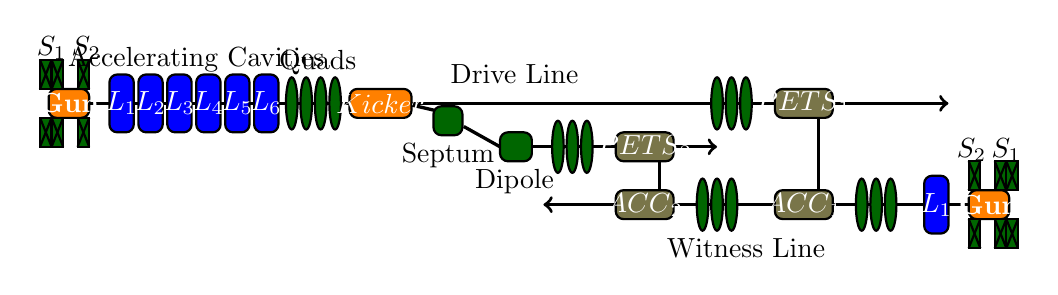
\begin{tikzpicture}[scale=\textwidth/33cm, text=black]
	%\begin{tikzpicture}[scale=0.5, text=black]
	\def \gunleft {-1.0}
\def \gunright {0.3}
\def \loneright {1.0}
\def \ltworight {2.0}
\def \lthreeright {3.0}
\def \lfourright {4.0}
\def \lfiveright {5.0}
\def \lsixright {6.0}
\def \quadone {7.3}
\def \quadfour{16}

\draw[very thick, ->] (0.0,1) -- (30,1);

\draw[fill=orange, thick, rounded corners =0.1cm] (\gunleft-0.1,0.5)rectangle (\gunright,1.5) node[pos=.5, white] {\textbf{Gun}} ;
%Straight through

%S1
\node[] at (-1,2.9) {$S_1$};
\draw[thick, fill=black!60!green] (-1.4,-0.5)rectangle  (-1.0,0.5) node[pos=.5, white] {} ;
\draw[black,  thick] (-1.4,-0.5) -- (-1.0,0.5);
\draw[black,  thick] (-1.4,0.5) -- (-1.0,-0.5);
\draw[ thick, fill=black!60!green] (-1.4,1.5)rectangle  (-1.0,2.5) node[pos=.5, white] {} ;
\draw[black,  thick] (-1.4,1.5) -- (-1.0,2.5);
\draw[black,  thick] (-1.4,2.5) -- (-1.0,1.5);

\draw[ thick, fill=black!60!green] (-1.0,-0.5)rectangle  (-0.6,0.5) node[pos=.5, white] {} ;
\draw[black,  thick] (-1.0,-0.5) -- (-0.6,0.5);
\draw[black,  thick] (-1.0,0.5) -- (-0.6,-0.5);
\draw[ thick, fill=black!60!green] (-1.0,1.5)rectangle  (-0.6,2.5) node[pos=.5, white] {} ;
\draw[black,  thick] (-1.0,1.5) -- (-0.6,2.5);
\draw[black,  thick] (-1.0,2.5) -- (-0.6,1.5);

%S2
\node[] at (0.2,2.9) {$S_2$};
\draw[ thick, fill=black!60!green] (-0.1,-0.5) rectangle  (0.3,0.5) node[pos=.5, white] {};
\draw[black,  thick] (-0.1,-0.5) -- (0.3,0.5);
\draw[black,  thick] (-0.1,0.5) -- (0.3,-0.5);
\draw[ thick, fill=black!60!green] (-0.1,1.5) rectangle  (0.3,2.5) node[pos=.5, white] {};
\draw[black,  thick] (-0.1,1.5) -- (0.3,2.5);
\draw[black,  thick] (-0.1,2.5) -- (0.3,1.5);
%Linac drawings 
\node[] at (4,2.5) {Accelerating Cavities};
\draw[fill=blue,  thick, rounded corners =0.1cm] (\loneright,0)rectangle  ({\loneright+0.84},2) node[pos=.5, white] {$L_1$} ;
\draw[fill=blue,  thick, rounded corners =0.1cm] (\ltworight,0)rectangle  ({\ltworight+0.84},2) node[pos=.5, white] {$L_2$};
\draw[fill=blue,  thick, rounded corners =0.1cm] (\lthreeright,0)rectangle ({\lthreeright+0.84},2) node[pos=.5, white] {$L_3$};
\draw[fill=blue,  thick, rounded corners =0.1cm] (\lfourright,0)rectangle ({\lfourright+0.84},2) node[pos=.5, white] {$L_4$};
\draw[fill=blue,  thick, rounded corners =0.1cm] (\lfiveright,0)rectangle ({\lfiveright+0.84},2) node[pos=.5, white] {$L_5$};
\draw[fill=blue,  thick, rounded corners =0.1cm] (\lsixright,0)rectangle ({\lsixright+0.84},2) node[pos=.5, white] {$L_6$};

%current optimization point
%\node[draw, fill=yellow, star, star points=5, star point ratio=0.6, minimum size=0.1cm]
%at (12.5,1.0) {$z_1$};


%Quad drawings
\node[] at (8.2,2.4) {Quads};
\draw[fill=black!60!green,  thick] (\quadone, 1.0) ellipse (0.2cm and 0.9cm);
\draw[fill=black!60!green,  thick] (\quadone+0.5, 1.0) ellipse (0.2cm and 0.9cm);
\draw[fill=black!60!green,  thick] (\quadone+1.0, 1.0) ellipse (0.2cm and 0.9cm);
\draw[fill=black!60!green,  thick] (\quadone+1.5, 1.0) ellipse (0.2cm and 0.9cm);

%Line between kicker and septum
\node[] at (15,2) {Drive Line};
\node[] at (23,-4) {Witness Line};
\draw[very thick] (\lsixright+5.2,1.0) -- (12.5,0.7);

%Kicker 
\draw[fill=orange,  thick, rounded corners =0.1cm] (\lsixright+3.3,0.5)rectangle ({\lsixright+0.84+4.6},1.5) node[pos=.5, white] {$Kicker$};

%Septum
\node[] at (12.7,-0.8) {Septum};
\draw[fill=black!60!green,  thick, rounded corners =0.1cm] (12.2,0.9)rectangle ({13.2},-0.1) node[pos=.5, white] {};
%\draw[latex-latex] (\gunleft,-5.0) -- (14,-5.0) ;
%\foreach \x in  {0.3, 1.0, 3.5, 5.0, 7.0, 8.5, 10, 12.5} %tick marks
%\draw[shift={(\x,-5.0)},color=black] (0pt,3pt) -- (0pt,-3pt);
%\foreach \x in {0.3, 1.0, 3.5, 5.0, 7.0, 8.5, 10, 12.5}
%\draw[shift={(\x,-5.2)},color=black] (0pt,0pt) node[below] {$\x$};

%Line between kicker and septum
\draw[very thick] (13.25,0.2) -- (14.5,-0.5);

%Dipole
\node[] at (15,-1.7) {Dipole};
\draw[fill=black!60!green, thick, rounded corners =0.1cm] (14.5,0.0)rectangle ({15.6},-1.0) node[pos=.5, white] {};

%Line between dipole and quads
\draw[very thick, ->] (15.6,-0.5) -- (22,-0.5);
%Second set of quads
\draw[fill=black!60!green,  thick] (\quadfour+0.5, -0.50) ellipse (0.2cm and 0.9cm);
\draw[fill=black!60!green,  thick] (\quadfour+1.0, -0.50) ellipse (0.2cm and 0.9cm);
\draw[fill=black!60!green,  thick] (\quadfour+1.5, -0.50) ellipse (0.2cm and 0.9cm);



\def \quadfive{22}
%Third set of quads
\draw[fill=black!60!green,  thick] (\quadfive, 1.0) ellipse (0.2cm and 0.9cm);
\draw[fill=black!60!green,  thick] (\quadfive+0.5, 1.0) ellipse (0.2cm and 0.9cm);
\draw[fill=black!60!green,  thick] (\quadfive+1.0, 1.0) ellipse (0.2cm and 0.9cm);


%Witness
\draw[very thick, <-] (16,-2.5) -- (31,-2.5);

%Waveguide
\draw[very thick] (20,-0.5) -- (20,-3);
%Waveguide
\draw[very thick] (25.5,1.5) -- (25.5,-3);

%PETS2
\draw[fill=black!60!yellow,  thick, rounded corners =0.1cm] (18.5,0.0)rectangle (20.5,-1) node[pos=.5, white] {$\text{PETS}_2$};
%PETS1
\draw[fill=black!60!yellow,  thick, rounded corners =0.1cm] (24,1.5)rectangle (26,0.5) node[pos=.5, white] {$\text{PETS}_1$};

%ACC2
\draw[fill=black!60!yellow,  thick, rounded corners =0.1cm] (18.5,-2)rectangle (20.5,-3) node[pos=.5, white] {$\text{ACC}_2$};
%ACC1
\draw[fill=black!60!yellow,  thick, rounded corners =0.1cm] (24,-2)rectangle (26,-3) node[pos=.5, white] {$\text{ACC}_1$};
\def \quadsix{27}
%Third set of quads
\draw[fill=black!60!green,  thick] (\quadsix, -2.5) ellipse (0.2cm and 0.9cm);
\draw[fill=black!60!green,  thick] (\quadsix+0.5, -2.5) ellipse (0.2cm and 0.9cm);
\draw[fill=black!60!green,  thick] (\quadsix+1.0, -2.5) ellipse (0.2cm and 0.9cm);
\def \quadseven{21.5}
%Third set of quads
\draw[fill=black!60!green,  thick] (\quadseven, -2.5) ellipse (0.2cm and 0.9cm);
\draw[fill=black!60!green,  thick] (\quadseven+0.5, -2.5) ellipse (0.2cm and 0.9cm);
\draw[fill=black!60!green,  thick] (\quadseven+1.0, -2.5) ellipse (0.2cm and 0.9cm);

\begin{scope}[yscale=1,xscale=-1, yshift=-3.5cm, xshift=-31cm]
	\draw[fill=orange, thick, rounded corners =0.1cm] (\gunleft-0.1,0.5)rectangle (\gunright,1.5) node[pos=.5, white] {\textbf{Gun}} ;
	
	%S1
	\node[] at (-1,2.9) {$S_1$};
	\draw[thick, fill=black!60!green] (-1.4,-0.5)rectangle  (-1.0,0.5) node[pos=.5, white] {} ;
	\draw[black,  thick] (-1.4,-0.5) -- (-1.0,0.5);
	\draw[black,  thick] (-1.4,0.5) -- (-1.0,-0.5);
	\draw[ thick, fill=black!60!green] (-1.4,1.5)rectangle  (-1.0,2.5) node[pos=.5, white] {} ;
	\draw[black,  thick] (-1.4,1.5) -- (-1.0,2.5);
	\draw[black,  thick] (-1.4,2.5) -- (-1.0,1.5);
	
	\draw[ thick, fill=black!60!green] (-1.0,-0.5)rectangle  (-0.6,0.5) node[pos=.5, white] {} ;
	\draw[black,  thick] (-1.0,-0.5) -- (-0.6,0.5);
	\draw[black,  thick] (-1.0,0.5) -- (-0.6,-0.5);
	\draw[ thick, fill=black!60!green] (-1.0,1.5)rectangle  (-0.6,2.5) node[pos=.5, white] {} ;
	\draw[black,  thick] (-1.0,1.5) -- (-0.6,2.5);
	\draw[black,  thick] (-1.0,2.5) -- (-0.6,1.5);
	
	%S2
	\node[] at (0.2,2.9) {$S_2$};
	\draw[ thick, fill=black!60!green] (-0.1,-0.5) rectangle  (0.3,0.5) node[pos=.5, white] {};
	\draw[black,  thick] (-0.1,-0.5) -- (0.3,0.5);
	\draw[black,  thick] (-0.1,0.5) -- (0.3,-0.5);
	\draw[ thick, fill=black!60!green] (-0.1,1.5) rectangle  (0.3,2.5) node[pos=.5, white] {};
	\draw[black,  thick] (-0.1,1.5) -- (0.3,2.5);
	\draw[black,  thick] (-0.1,2.5) -- (0.3,1.5);
	%Linac drawings 
	%\node[] at (4,2.5) {Accelerating Cavities};
	\draw[fill=blue,  thick, rounded corners =0.1cm] (\loneright,0)rectangle  ({\loneright+0.84},2) node[pos=.5, white] {$L_1$} ;
	
\end{scope}



	\end{tikzpicture}
	\caption{TBA beam line layout at the AWA. The arrow at the end of each line indicates what direction the beam is traveling.
		PETS stands for Power Extraction and Transfer Structure, and ACC
		stands for Accelerating structure. The subscript index on each structure refers to which stage the structures belong to, first or second stage. }
	\label{beamline}
\end{figure*}

The kicker will ensure that one bunch train is supplied to 
each stage. This allows for more energy transfer in stage 2.
If the same bunch train supplies both stages \cite{tba}, the amount
of available energy for stage 2 would be decreased by the 
amount of energy deposited in stage 1. This would cause
unequal energy gain in each stage.
After passing the kicker, 
the high charge bunch trains are supplied to Power Extraction
and Transfer Structures (PETS) downstream. These are decelerating 
structures that extract power from the bunches through wakefield generation.
The structures take advantage of superposition and allow the wake from each 
bunch to combine to the others. A high power pulse is generated by 
the combination of wakes and transfered through a waveguide to the 
witness line. 
There are two decelerating stages on the drive line, and two 
corresponding accelerating sections on the witness line.
The accelerating structures, ACC$_1$ and ACC$_2$, are only 
powered by the PETS on the drive line. There is no  
external power source. 

\subsection{Stage 1}
The first accelerating stage refers to portions of the beam line that 
support ACC$_1$, and PEST$_1$. This is the straight 
through portion of the drive beam line. The first bunch train will be allowed
to pass the kicker when it is unactivated, i.e. not pulse and no field present.
The bunch train will then arrive at the quadrupoles before PETS$_1$. 
Focusing will ensure maximum transmission of the \SI{40}{nC} 
bunch train through PEST$_1$. Integrated Current Transformers (ICT's), 
are located before and after all PETS and ACC structures to monitor the 
transmission.   
\begin{figure}
	\begin{tikzpicture}[every node/.style={anchor=south west,inner sep=0pt},x=1mm, y=1mm,]   
	\node (fig1) at (0,0)
	{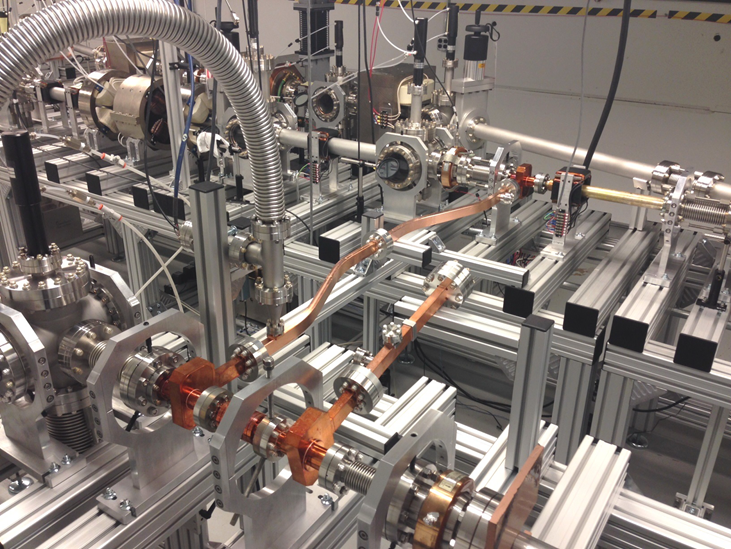
\includegraphics[width=0.5\textwidth]{stage}};
	\node[fill=white, inner sep=2pt] (txt2) at (15,10) {ACC};
	\node[fill=white, inner sep=2pt] (txt2) at (66,35) {PETS};
	\node[fill=white, inner sep=2pt, rotate=32] (txt2) at (35,33) {Waveguide};
	\end{tikzpicture}
	\caption{Example of a TBA stage at the AWA. This picture was taken during 
	metallic TBA experiment \cite{tba}. }
	\label{stage}
\end{figure}

Although not shown in Fig~\ref{beamline}, 
a spectrometer will be located at the end of the line. Energy loss
in the bunch train will serve as a way to infer how much power was
deposited in the PETS$_1$. Energy measurements in combination
with rf probe measurements in the transfer waveguide and ACC$_1$,
will be used to calculate losses in the stage. 

\subsection{Stage 2}
Likewise, stage 2 supports ACC$_2$ and PETS$_2$. After the first 
bunch train passes the kicker and goes on to PETS$_1$, 
the kicker will be pulsed. The second
bunch train will be directed to the bent beam line on drive side.
Meanwhile the same bunch on the witness side that was accelerated in 
stage 1 will arrive at stage 2, receiving a second increase in energy.
Successful energy gain in both stages is key to demonstrating staged TBA.
A second spectrometer will be located at the end of the bent beam line.
There will also be a second set of spectrometers on the witness line.


\section{Synchronization}
The rf power generated on the drive line
must reach the accelerating structures as the witness beam is arriving.
This requires understanding of the laser trigger, 
bunch train spacing, beams travel time, 
rise time of the rf pulse generated in the PETS, 
travel time of the pulse in the waveguide, and 
the fill time needed in the accelerating structures. 
While implementing this level of synchronization is not trivial, 
it possible, and has been demonstrated in previous experiments
at the AWA \cite{tba}. 

To understand this timing, we must start with the UV laser.
Both the drive and witness line electron bunches
originate from the same ultraviolet (UV) laser pulse. 
A network of UV optics and splitters deliver one laser 
pulse to the witness gun, and a pulse train to the drive gun \cite{korea}.
Each UV pulse is \SI{769}{ps} long, which is one wavelength ($\lambda$)
of the \SI{1.3}{GHz} rf operating frequency of the beam line.  
An additional wavelength is used as spacing between each bunch train.
This brings the length of an eight bunch train to $15\lambda$ or about \SI{11.5}{ns}.
Since only one bunch is send to the witness line, the length of the 
laser pulse on the witness line is only $1\lambda$.

The bunch train must travel a longer distance to reach PETS$_1$ 
than the distance the witness bunch must travel to reach ACC$_1$.
The the difference in travel time is accounted for by adding an optical delay 
to the UV optics proceeding the witness gun. 
[ADD MORE HERE ABOUT TIMING...]


\section{Kicker}
A kicker was specifically fabricated 
for this experiment. The initial design was adapted from 
work done at Indiana University \cite{kicker,korea}. The plates were lengthened
to increase the angle and the gap adjusted based on 
beam size simulations and mechanical constraints at the AWA. 
The design specifications and final kicker parameters 
are shown in Table~\ref{tkick}. The plates will be 
operated in differential mode, to get the highest field
possible from the available pulsar.
\begin{table}[hbt]
	%   \vspace*{-.5\baselineskip}
	\centering
	\caption{Final Kicker Parameters}
	\begin{tabular}{lc}
		\toprule
		\textbf{Parameter} & \textbf{Value} \\
		\midrule
		Charge       		& \SI{40}{nC}   \\ %[3pt]
		Beam Energy  		& \SI{70}{MeV}  \\ %[3pt]
		Angle 	     		& $2^{\circ}$ 	\\
		Gap Between Plates  & \SI{40}{mm}	\\		 
		Length of Plates    & \SI{500}{A}	\\
		Pulsar Voltage      & $\pm$\SI{24}{kV} \\
		Field Rise Time  	& \SI{3}{ns}    \\
		Min Field Duration 	& \SI{12}{ns}  \\ %[3pt]
		\bottomrule
	\end{tabular}
	\label{tkick}
	%   \vspace*{-\baselineskip}
\end{table}

After fabrication, a high voltage test was performed to ensure 
the electrical feedthroughs were sound. Special thanks to 
the Power Systems group at the Advanced Photon Source (APS) for testing 
the kicker in one of their rf cages, see Fig.~\ref{cage}
A high voltage \SI{60}{Hz} 
source was used to probe one blade of the kicker at a time. 
Both sides performed well, with one blade showing slight discharge
at \SI{8}{KV} RMS, and the other showing no discharge up to \SI{9}{KV} RMS
(the limit of the source). These results are in line with other kickers
designed and tested at the APS \cite{mbakicker}.  

\begin{figure}
	\begin{tikzpicture}[every node/.style={anchor=south west,inner sep=0pt},x=1mm, y=1mm,]   
	\node (fig1) at (0,0)
	{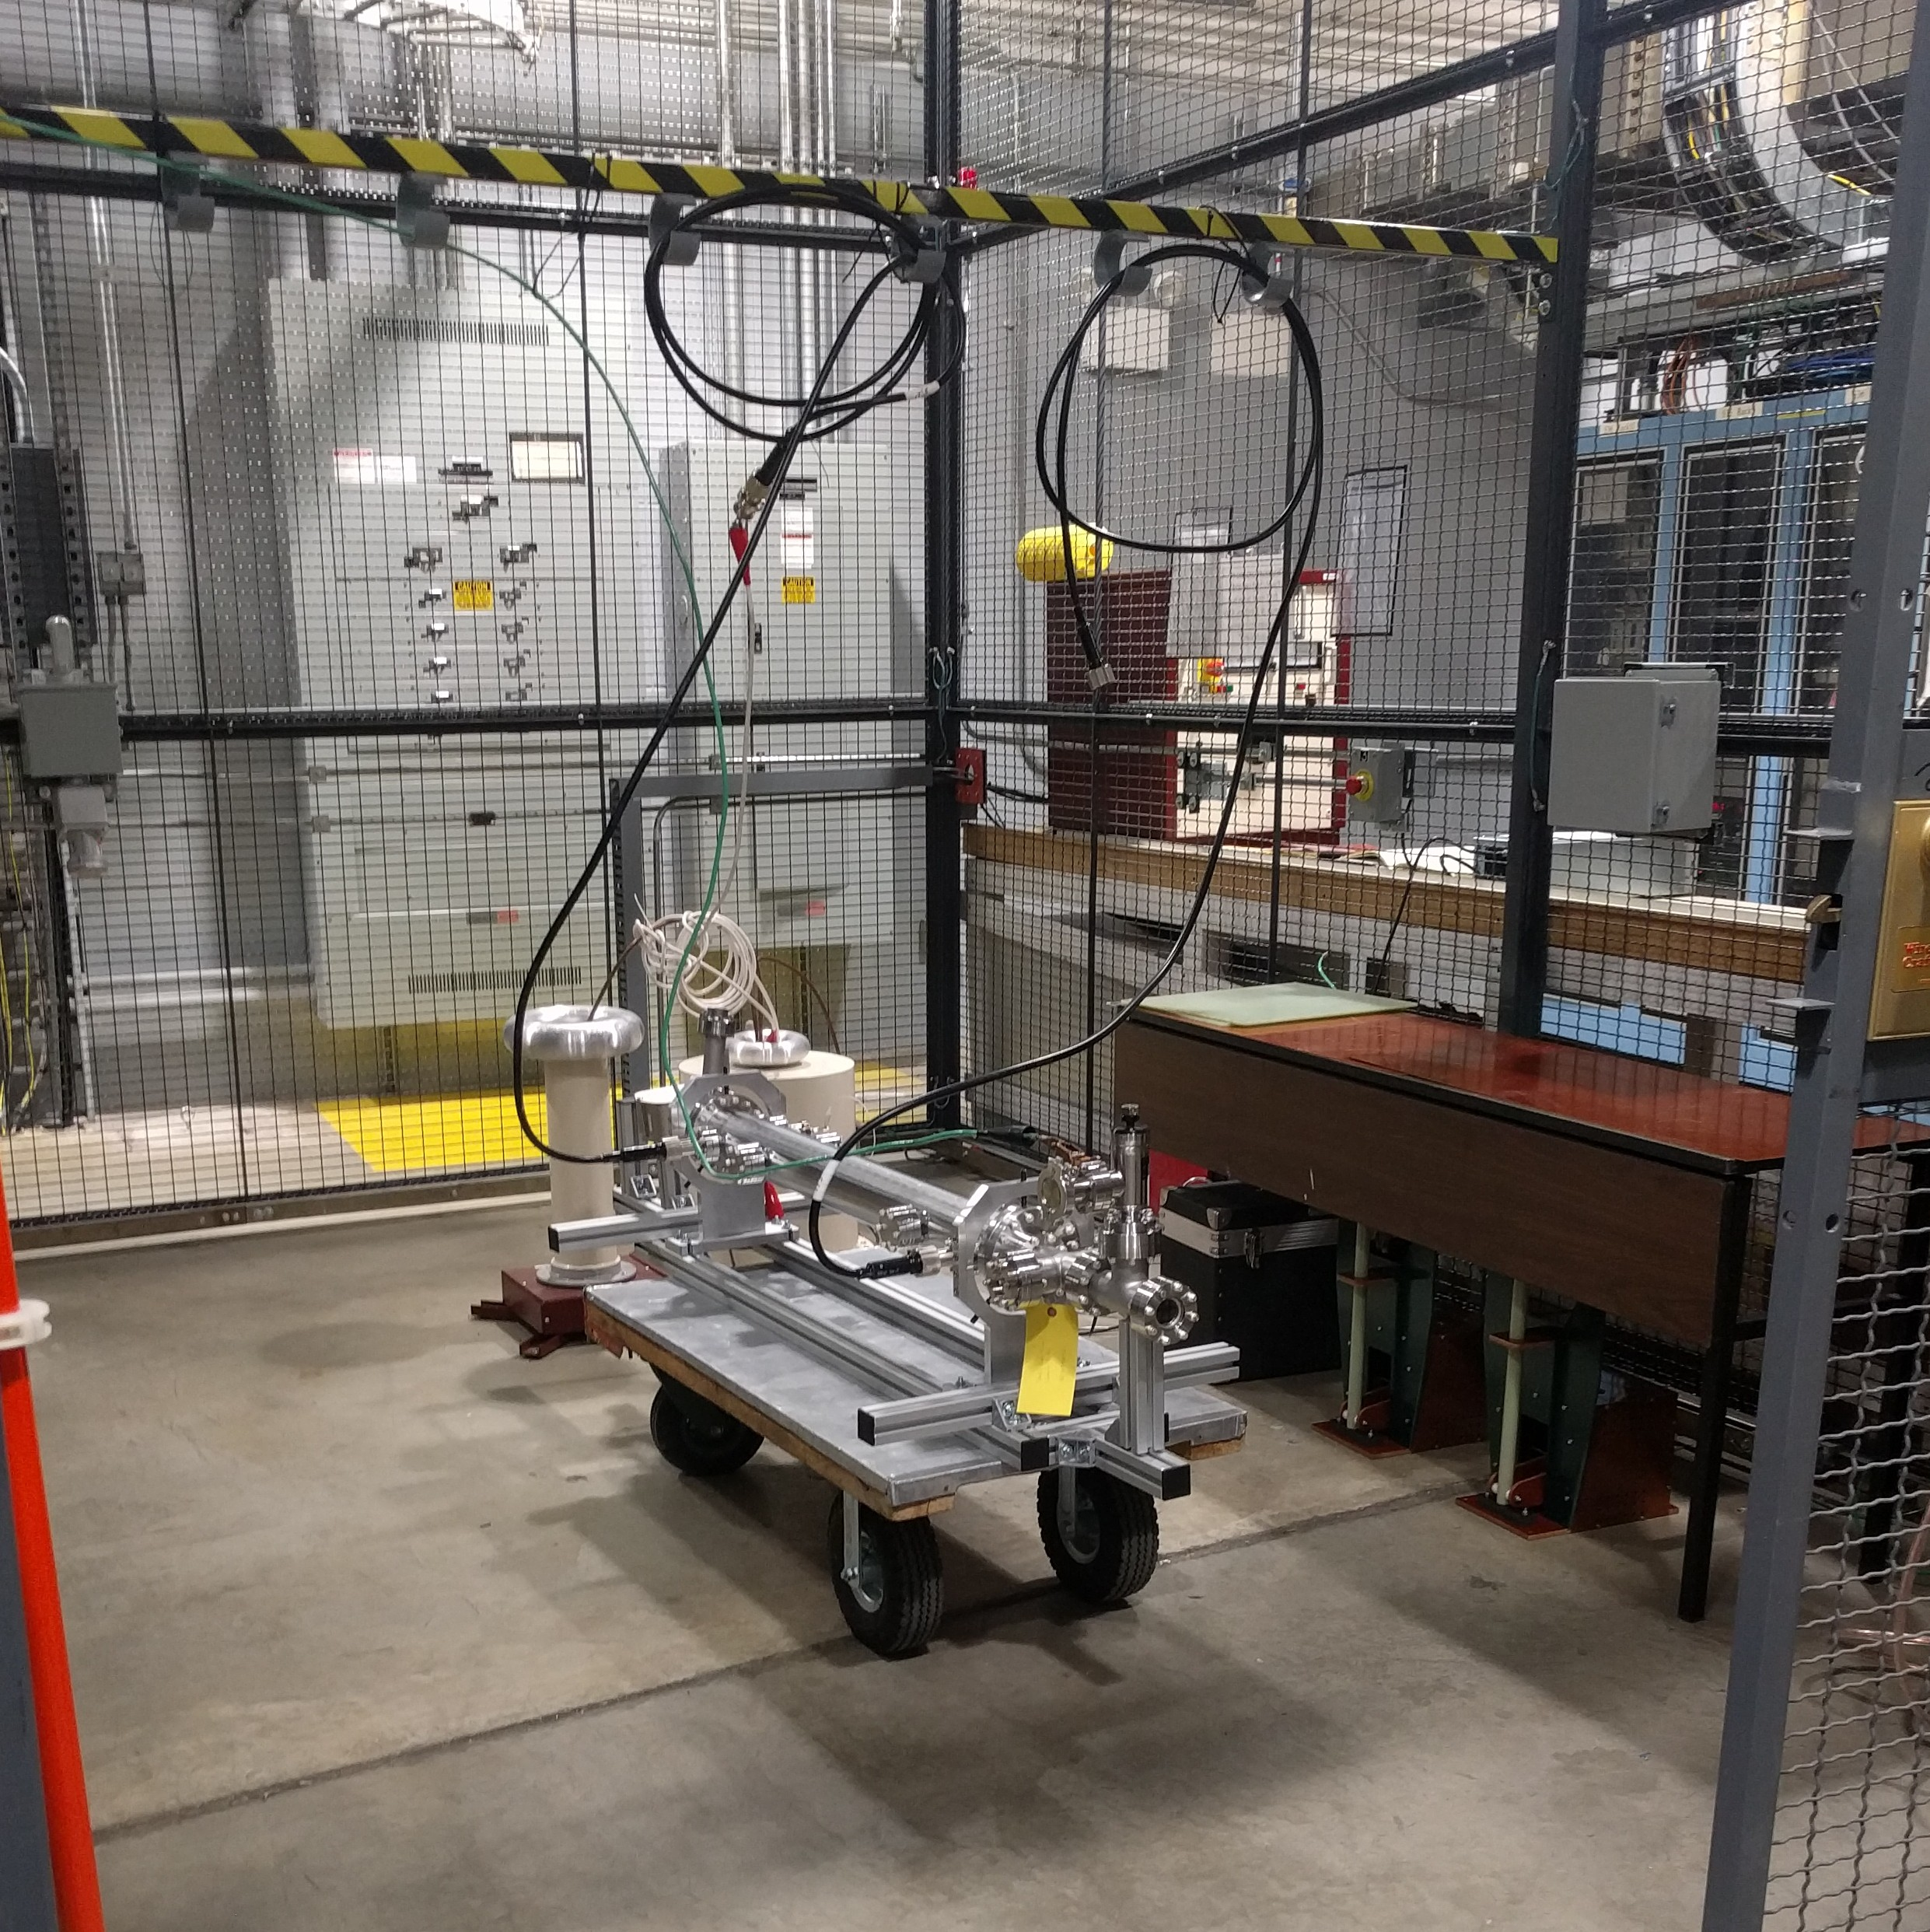
\includegraphics[width=0.5\textwidth]{kicker-hv}};
	\node[fill=white, inner sep=2pt] (txt2) at (40,15) {Kicker};
	\node[fill=white, inner sep=2pt] (txt2) at (10,45) {HV Source};
	\end{tikzpicture}
	\caption{Kicker in high voltage (HV) testing cage at the Advanced Photon Source. }
	\label{cage}
\end{figure}

\section{Ongoing Optimization}
While the number of optics elements and their 
general locations is known, there are still many free parameters that 
are not determined by that information alone. 
The strength of each magnet, the phase in each cavity, 
and the laser profile can all be freely adjusted.
This leads to a high dimensional optimization problem. 
The parameters on the drive line are further complicated
by strong space charge forces and bending elements (kicker, septum, dipole).

A first round multi-objective optimization of the drive line has been performed 
using the built in genetic algorithm (GA) in OPAL-T \cite{opal}. 
These simulations included the gun and all elements leading up 
to the entrance of the septum, as shown in Fig.~\ref{beamline}.
The objectives were beam size, emittance, and energy spread before the kicker.
Simulation parameters are shown in Table~\ref{simparam}.
Results of this optimization work will be published soon.
[Leave it at that? I don't want to add anything that will be in the paper]
\begin{table}[hbt]
	%   \vspace*{-.5\baselineskip}
	\centering
	\caption{Drive Line Simulation Parameters}
	\begin{tabular}{lcc}
		\toprule
		\textbf{Parameter} & \textbf{Fixed Value}  & \textbf{Optimization Values} \\
		\midrule
		Charge       & \SI{40}{nC}       & --   \\ %[3pt]
		Gun Gradient & \SI{65}{MV/m}     & --  \\ %[3pt]
		Laser Radius & \SI{9}{mm}        & --    \\
		Laser FWHM   & --      			 & \SI{1.5}{ps} $\leq F \leq $ \SI{10}{ps}	  \\ %[3pt]
		Gun Phase    & -- 				 & \SI{-20}{}$^{\circ} \leq \phi_g \leq$ \SI{0}{}$^{\circ}$  \\	
		Linac Phases & --		         & \SI{-20}{}$^{\circ} \leq \phi_l \leq$ \SI{0}{}$^{\circ}$ 	  \\	 
		$S_1$        & --		 		 & \SI{300}{A} $\leq B \leq $ \SI{500}{A}	  \\
		$S_2$		 & --  	 			 & \SI{180}{A} $\leq M \leq $ \SI{280}{A}	  \\
		\bottomrule
	\end{tabular}
	\label{simparam}
	%   \vspace*{-\baselineskip}
\end{table}


\section{Conclusion}
The TBA layout for upcoming experiments at the 
AWA facility is approximately decided. A fast rise time kicker
was designed and fabricated for this experiment. 
A high voltage test was preformed at the 
Advanced Photon Source. Initial optimization 
work has been done to decide  
optics parameters for the high charge drive line.
Additional design work and optimization studies will be done 
to finalize the optics further downstream. 

\section{acknowledgments}
We gratefully acknowledge the computing resources
provided on Bebop, a high-performance computing cluster
operated by the LCRC at Argonne National Laboratory.
This material is based upon work supported by the 
U.S. Department of Energy, Office of Science, under 
contract number DE-AC02-06CH11357 and grant number DE-SC0015479. 
Travel to IPAC'18 supported by the Division of Physics 
of the United States National Science Foundation 
Accelerator Science Program and the Division of 
Beam Physics of the American Physical Society.


\begin{thebibliography}{9}
\bibitem{eex}
G.~Ha \emph{et al.}, “Demonstration of Current Profile 
Shaping using Double Dog-Leg Emittance Exchange Beam 
Line at Argonne Wakefield Accelerator”
in \textit{Proc. IPAC’16}, 
Busan, South Korea, May 2016, 
paper TUOBB01.

\bibitem{pets}
J.~Shao \emph{et al.}, 
“Recent Progress towards Dielectric Short Pulse Two-Beam Acceleration”
in \textit{Proc. IPAC’18}, 
Vancouver, Canada, May 2018, 
paper TUYGBE3.

\bibitem{therm}
L.~Zheng \emph{et al.}, “Measurements of Thermal Emittance 
for Cesium Telluride Photocathodes in an L-Band RF Gun”
in \textit{Proc. IPAC’17}, 
Copenhagen, Denmark, May 2017, 
paper TUPAB074.

\bibitem{tba}
J.~Shao \emph{et al.}, “Recent Two-Beam 
Acceleration Activities at Argonne Wakefield Accelerator Facility”
in \textit{Proc. IPAC’17}, 
Copenhagen, Denmark, May 2017, 
paper WEPVA022.

\bibitem{kicker}
T.~H.~Luo \emph{et al.}, “Design of a Fast
Extraction Kicker for the ALPHA Project”
in \textit{Proc. IPAC’10}, 
Kyoto, Japan, May 2010, 
paper THPEA052.

\bibitem{korea}
N.~Neveu \emph{et al.}, 
“Drive Generation and Propagation Studies for the Two
Beam Acceleration Experiment at the Argonne Wakefield
Accelerator,”
in \emph{Proc. IPAC'16}, 
Busan, South Korea, May 2016, 
paper TUPMY036.

\bibitem{mbakicker}
C.~Yao \emph{et al.}, 
“Development of Fast Kickers for the APS
MBA Upgrade,”
in \emph{Proc. IPAC'15}, 
Richmond, VA, USA, May 2015, 
paper WEPTY014.



\bibitem{opal}
A.~Adelmann \emph{et al.},
“The OPAL (Object Oriented Parallel Accelerator Library) framework,”
PSI, Zurich, Switzerland,
Rep. PSI-PR-08-02, 2008-2017.

\bibitem{fish}
\emph{Reference Manual for the POISSON/SUPERFISH Group of 
	Codes},  Los Alamos Accelerator Code Group,  
 Los Alamos, NM, USA, 
 Rep. LA-UR-87-126, Jan. 1987.
\end{thebibliography}

\end{document}
	
